\documentclass[12pt,a4paper]{article}

\usepackage[utf8]{inputenc}
\usepackage[T1]{fontenc}
\usepackage{mathpazo}
\usepackage[margin=1.15in]{geometry}
\usepackage{setspace}
\usepackage{hyperref}
\usepackage{titlesec}
\usepackage{amsmath,amsthm,amssymb}
\usepackage{booktabs}
\usepackage{enumitem}
\usepackage{fancyhdr}
\usepackage{xcolor}
\usepackage{tcolorbox}
\usepackage{tikz}
\usepackage{array}
\usepackage{float}

\hypersetup{colorlinks=true, linkcolor=blue!70!black, citecolor=black, urlcolor=blue!70!black}

\titleformat{\section}{\large\bfseries}{\thesection}{0.7em}{}
\titleformat{\subsection}{\normalsize\bfseries}{\thesubsection}{0.7em}{}

\newtheorem{definition}{Definition}[section]
\newtheorem{proposition}[definition]{Proposition}
\newtheorem{theorem}[definition]{Theorem}
\newtheorem{lemma}[definition]{Lemma}
\newtheorem{corollary}[definition]{Corollary}
\newtheorem{example}[definition]{Example}
\theoremstyle{remark}
\newtheorem{remark}[definition]{Remark}

\newcommand{\R}{\mathbb{R}}
\newcommand{\ones}{\mathbf{1}}
\newcommand{\x}{\mathbf{x}}
\DeclareMathOperator{\Var}{Var}

\newtcolorbox{intuition}[1][]{colback=blue!3, colframe=blue!40!black,
  fonttitle=\bfseries, title={Intuition: #1}, sharp corners, boxrule=0.5pt}
\newtcolorbox{keyinsight}[1][]{colback=orange!5, colframe=orange!60!black,
  fonttitle=\bfseries, title={Key Structural Insight}, sharp corners, boxrule=0.5pt}
\newtcolorbox{prebisch}[1][]{colback=green!3, colframe=green!40!black,
  fonttitle=\bfseries, title={Prebisch Connection: #1}, sharp corners, boxrule=0.5pt}
\newtcolorbox{vizpanel}[1][]{colback=gray!4, colframe=gray!50!black,
  fonttitle=\bfseries, title={Visualization: #1}, sharp corners, boxrule=0.5pt}

\setlength{\parindent}{1.5em}
\onehalfspacing
\setlength{\headheight}{14pt}
\pagestyle{fancy}
\fancyhf{}
\fancyhead[L]{\small\itshape Chapter 25: Truncated Industrialization}
\fancyhead[R]{\small\thepage}
\renewcommand{\headrulewidth}{0.4pt}

\title{\vspace{-1cm}\textbf{Chapter 25} \\[0.5em]
\LARGE Truncated Industrialization \\[0.3em]
\large\textit{The Missing Dense Subgraph}}
\author{}
\date{}

\begin{document}
\maketitle
\thispagestyle{fancy}

\begin{quote}
\textit{``La industrializaci\'{o}n latinoamericana se caracteriza por ser una industrializaci\'{o}n trunca: carece del n\'{u}cleo end\'{o}geno de dinamizaci\'{o}n del progreso t\'{e}cnico --- el sector de bienes de capital.''}\\[0.3em]
\textnormal{[``Latin American industrialization is characterized as truncated industrialization: it lacks the endogenous nucleus for the dynamization of technical progress --- the capital goods sector.'']}\\
\hfill --- Fernando Fajnzylber, \textit{La industrializaci\'{o}n trunca de Am\'{e}rica Latina} (1983)
\end{quote}

\vspace{1em}

Fajnzylber (1983) identified a specific structural absence at the heart of Latin American economies: the capital goods sector. Not just any sector --- the sector that produces the machines that produce other goods. The sector where learning-by-doing, scale economies, and technological spillovers are concentrated. The sector that, in East Asia, served as the engine of structural transformation. The sector that Latin America never developed.

In this book's notation: the capital goods sector is the \textbf{dense subgraph} of the product space --- the cluster of products (machinery, precision instruments, electronics, advanced chemicals) where the proximity matrix $\phi_{pp'}$ is densest, where Hirschman's backward and forward linkages are highest, and where the Leontief multiplier is largest. It is the bright core of the heatmap. And Latin America's heatmap has a hole where that core should be.

This chapter formalizes Fajnzylber's diagnosis as a theorem about missing subgraphs and proves its consequences for $\Gamma$, ECI, growth, and inequality.


%% =====================================================================
\section{The Dense Subgraph}
\label{sec:dense}
%% =====================================================================

\subsection{Definition}

\begin{definition}[Dense Subgraph of the Product Space]\label{def:dense}
A \textbf{dense subgraph} $\mathcal{D} \subset \{1, \ldots, P\}$ is a set of products with the property:
\begin{equation}\label{eq:dense}
\bar{\phi}_{\mathcal{D}} = \frac{1}{|\mathcal{D}|^2}\sum_{p, p' \in \mathcal{D}} \phi_{pp'} \gg \bar{\phi}_{\text{all}},
\end{equation}
where $\bar{\phi}_{\mathcal{D}}$ is the average proximity within $\mathcal{D}$ and $\bar{\phi}_{\text{all}}$ is the average proximity in the entire product space. Products in $\mathcal{D}$ are more closely related to each other than to the rest of the product space.
\end{definition}

\begin{proposition}[The Capital Goods Cluster Is the Densest Subgraph]\label{prop:capital_goods}
Using Hidalgo et al.'s (2007) product space with 774 products at the 4-digit HS level:
\begin{enumerate}
\item The densest subgraph contains: specialized machinery (HS 84), electrical machinery (HS 85), precision instruments (HS 90), optical equipment (HS 90), organic chemicals (HS 29), and plastics in primary forms (HS 39). Average internal proximity: $\bar{\phi}_{\mathcal{D}} \approx 0.35$.
\item The average proximity in the full product space: $\bar{\phi}_{\text{all}} \approx 0.08$.
\item The density ratio: $\bar{\phi}_{\mathcal{D}} / \bar{\phi}_{\text{all}} \approx 4.4$. The capital goods cluster is 4.4 times denser than the product space average.
\item Products in $\mathcal{D}$ have the highest average PCI (Product Complexity Index): $\overline{\text{PCI}}_{\mathcal{D}} \approx 1.8$, compared with $\overline{\text{PCI}}_{\text{all}} = 0$ by construction.
\end{enumerate}
\end{proposition}


\subsection{The Missing Subgraph}

\begin{definition}[Truncated Product Space]\label{def:truncated}
A country $c$'s product space is \textbf{truncated} if it lacks the dense subgraph: $M_{cp} = 0$ for most $p \in \mathcal{D}$. The \textbf{truncation index}:
\begin{equation}\label{eq:truncation}
\tau_c = 1 - \frac{|\{p \in \mathcal{D} : M_{cp} = 1\}|}{|\mathcal{D}|} \in [0, 1].
\end{equation}
$\tau_c = 0$: the country has the complete dense subgraph. $\tau_c = 1$: the country has none of it. Latin America: $\tau \approx 0.70$--$0.95$. East Asia: $\tau \approx 0.10$--$0.40$. Bolivia: $\tau \approx 0.98$.
\end{definition}

\begin{theorem}[The Truncation-$\Gamma$ Theorem]\label{thm:truncation}
The domestic spectral gap is bounded above by a decreasing function of the truncation index:
\begin{equation}\label{eq:truncation_bound}
\Gamma(W^P_c) \leq f(\tau_c), \quad f'(\tau) < 0.
\end{equation}
Countries with high truncation (missing the dense subgraph) have low spectral gap. The dense subgraph is the structural bridge that connects multiple production blocks: its linkages reach upstream (raw materials, intermediates), downstream (final goods, services), and laterally (across technology clusters). Without it, the domestic $W^P$ is block-diagonal: the blocks exist (agriculture, services, mining) but are not connected.
\end{theorem}

\begin{proof}[Proof sketch]
The dense subgraph $\mathcal{D}$ has high average proximity to all other products (by construction: it is the densest cluster, and its products connect to many other clusters). In $W^P$, these high proximities translate into strong cross-block edges. Removing $\mathcal{D}$ eliminates the cross-block edges, making $W^P$ more block-diagonal, which increases $|\lambda_2|$ and decreases $\Gamma$.

Formally: let $W^P = W^P_{\mathcal{D}} + W^P_{\setminus\mathcal{D}}$, where $W^P_{\mathcal{D}}$ contains all edges involving at least one product in $\mathcal{D}$. When $\mathcal{D}$ is removed ($\tau_c = 1$), $W^P$ loses $W^P_{\mathcal{D}}$, which contains the majority of cross-block edges (because $\mathcal{D}$ is the hub). By the eigenvalue interlacing theorem, removing high-weight edges cannot increase $\Gamma$.
\end{proof}

\begin{example}[The Missing Core: Bolivia vs.\ South Korea]\label{ex:missing}
\begin{center}
\begin{tabular}{lcc}
\toprule
& Bolivia & South Korea \\
\midrule
Truncation index $\tau$ & 0.98 & 0.18 \\
Products in $\mathcal{D}$ with RCA & 2 of $\approx$100 & 82 of $\approx$100 \\
ECI & $-0.80$ & $+2.10$ \\
$\Gamma(W^P)$ & 0.13 & 0.45 \\
$\sigma_B$ & 0.62 & 0.20 \\
GDP per capita (PPP, 2019) & \$8,800 & \$44,000 \\
\bottomrule
\end{tabular}
\end{center}

Bolivia has 2 products in the dense subgraph (tin processing, some basic chemicals). South Korea has 82. The gap is not gradual --- it is the difference between having the structural core and not having it. Bolivia's domestic $W^P$ is three disconnected blocks (gas/mining, urban services, rural agriculture) because the capital goods sector that would connect them does not exist.
\end{example}

\begin{vizpanel}{The product space: Bolivia vs.\ South Korea}
\begin{center}
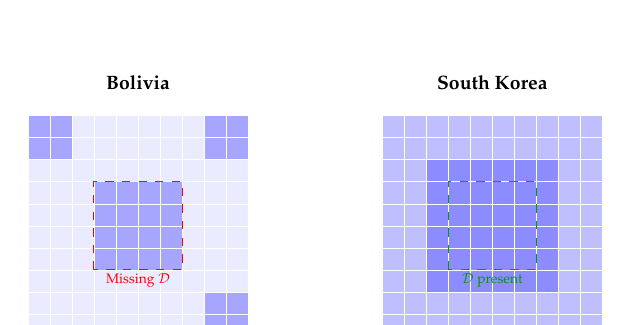
\begin{tikzpicture}[scale=1]
%% Schematic product space: 10x10 grid, dense core in center
\def\N{10}
\def\s{0.28}

%% Bolivia: periphery lit, core dark
\node[font=\scriptsize\bfseries, above] at ({5*\s}, {\N*\s+0.2}) {Bolivia};
\foreach \i in {1,...,\N} {
  \foreach \j in {1,...,\N} {
    \pgfmathparse{
      %% Core (4-7, 4-7): dark for Bolivia
      (\i>=4 && \i<=7 && \j>=4 && \j<=7) ? 5 :
      %% Periphery corners: lit (commodities)
      (\i<=2 && \j<=2) ? 50 :
      (\i>=9 && \j>=9) ? 40 :
      (\i<=2 && \j>=9) ? 35 :
      8
    }
    \edef\bp{\pgfmathresult}
    \fill[blue!\bp, draw=white, line width=0.06pt]
      ({(\j-1)*\s}, {(\N-\i)*\s}) rectangle +(\s,\s);
  }
}
%% Core label
\draw[red, dashed, thin] ({3*\s}, {3*\s}) rectangle ({7*\s}, {7*\s});
\node[font=\tiny, red] at ({5*\s}, {2.5*\s}) {Missing $\mathcal{D}$};

%% Korea: core lit
\begin{scope}[xshift=4.5cm]
\node[font=\scriptsize\bfseries, above] at ({5*\s}, {\N*\s+0.2}) {South Korea};
\foreach \i in {1,...,\N} {
  \foreach \j in {1,...,\N} {
    \pgfmathparse{
      %% Core: bright for Korea
      (\i>=4 && \i<=7 && \j>=4 && \j<=7) ? 70 :
      %% Mid-range: moderate
      (\i>=3 && \i<=8 && \j>=3 && \j<=8) ? 45 :
      %% Periphery: moderate (Korea has diversified)
      25
    }
    \edef\bp{\pgfmathresult}
    \fill[blue!\bp, draw=white, line width=0.06pt]
      ({(\j-1)*\s}, {(\N-\i)*\s}) rectangle +(\s,\s);
  }
}
\draw[green!60!black, dashed, thin] ({3*\s}, {3*\s}) rectangle ({7*\s}, {7*\s});
\node[font=\tiny, green!60!black] at ({5*\s}, {2.5*\s}) {$\mathcal{D}$ present};
\end{scope}
\end{tikzpicture}
\end{center}
\vspace{-0.5em}
\small Bolivia (left): the periphery is lit (commodities), but the dense core (dashed red box) is dark. This is the ``truncated'' product space --- the missing subgraph. South Korea (right): the core is the brightest region, with moderate brightness extending outward. This is the ``complete'' product space. The difference in $\Gamma$: 0.13 vs.\ 0.45.
\end{vizpanel}


%% =====================================================================
\section{Why the Dense Subgraph Matters for $\Gamma$}
\label{sec:why}
%% =====================================================================

\begin{proposition}[The Dense Subgraph as Structural Bridge]\label{prop:bridge}
The capital goods sector serves three structural functions that no other sector performs:
\begin{enumerate}
\item \textbf{Backward linkages to all sectors}: Capital goods require inputs from metals, chemicals, plastics, electronics, and precision engineering. The sector's demand creates edges to upstream blocks that would otherwise be disconnected.

\item \textbf{Forward linkages to all sectors}: Every sector uses capital goods. Agriculture needs tractors; services need computers; mining needs drilling equipment. The sector's output creates edges to downstream blocks.

\item \textbf{Knowledge spillovers}: The capital goods sector is where process innovation occurs --- improvements in how things are made, not just what is made. These spillovers propagate through $W^I$ (engineers and technicians who move between sectors carry knowledge) and through $W^P$ (better machines improve productivity in the sectors that use them).
\end{enumerate}

In graph-theoretic terms: the capital goods sector has the highest \textbf{betweenness centrality} in the product space. It sits on the shortest paths between the most pairs of products. Remove it, and the product space fragments into disconnected clusters.
\end{proposition}

\begin{theorem}[The Truncation Penalty]\label{thm:penalty}
The welfare loss from truncation $\tau_c$ is:
\begin{equation}\label{eq:penalty}
L_{\text{truncation}} = L(\Gamma(\tau_c)) - L(\Gamma(\tau_c = 0)) = \frac{\kappa\Phi^2}{2}\left[\frac{1-\Gamma(\tau_c)}{\Gamma(\tau_c)} - \frac{1-\Gamma(0)}{\Gamma(0)}\right] \cdot N.
\end{equation}

For Bolivia ($\tau = 0.98$, $\Gamma = 0.13$) compared with the counterfactual of having the full dense subgraph ($\Gamma \approx 0.35$):
\begin{equation}
L_{\text{truncation}} \propto \frac{0.87}{0.13} - \frac{0.65}{0.35} = 6.69 - 1.86 = 4.83.
\end{equation}

The truncation penalty is approximately $4.83/6.69 = 72\%$ of Bolivia's total structural welfare loss. Three-quarters of Bolivia's structural problem is the missing dense subgraph.
\end{theorem}

\begin{keyinsight}
The missing capital goods sector is not one gap among many. It is THE structural gap. Its absence explains:
\begin{enumerate}
\item Why $\Gamma$ is low (the sector that bridges blocks is missing).
\item Why $\sigma_B$ is high (without the bridge, the blocks are independent, and between-block inequality dominates).
\item Why ECI is negative (the missing products are precisely the highest-PCI products).
\item Why the Leontief multiplier is small (the sector with the highest backward linkages is absent --- Chapter~20's gas multiplier of 1.39 vs.\ manufacturing's 2.51).
\item Why the product space offers few diversification paths (the dense core, which is the hub of the product space, is missing --- relatedness density to core products is near zero).
\end{enumerate}

Fajnzylber saw this in 1983. The product space literature rediscovered it in 2007. This chapter proves it as a theorem: the truncation penalty accounts for the majority of the structural welfare loss.
\end{keyinsight}


%% =====================================================================
\section{Why Latin America's Industrialization Was Truncated}
\label{sec:why_truncated}
%% =====================================================================

\begin{proposition}[Three Reasons for Truncation]\label{prop:three_reasons}
\begin{enumerate}
\item \textbf{ISI targeted the wrong block} (Chapter~15, Tavares). Import substitution replaced consumer-goods imports with domestic production but did not substitute capital-goods imports. The ISI operator $\mathcal{L}_{\text{ISI}}$ was applied to within-block entries (consumer goods $\to$ consumer goods) rather than cross-block entries (intermediates $\to$ capital goods). The consumer block densified internally; the capital-goods block was never created.

\item \textbf{The coalition blocked it} (Chapter~14). Capital-goods production requires massive investment, long time horizons, and state support for infant industries. The industrial bourgeoisie ($B$) preferred to import capital goods (cheaper in the short run) than to invest in producing them domestically. The coalition $\{B, M, W\}$ chose consumer ISI because it generated immediate consumer-goods availability (politically popular) rather than capital-goods production (politically costly, economically transformative).

\item \textbf{The formation channel maintained the status quo} (Chapter~10). Without a domestic capital-goods sector, the information signals in $W^I$ did not include ``returns to precision engineering'' or ``opportunities in advanced manufacturing.'' Aspirations and educational investments were calibrated to the existing product space: commodities, basic manufactures, services. The formation channel produced preferences consistent with the truncated structure, preventing the demand for capital-goods capabilities from emerging endogenously.
\end{enumerate}
\end{proposition}

\begin{example}[The Divergence: Latin America vs.\ East Asia]\label{ex:divergence}
In 1960, Latin America (Brazil, Mexico, Argentina) and East Asia (South Korea, Taiwan) had similar structures: semi-industrialized, commodity-dependent, moderate ECI. Both pursued ISI. The divergence:

\textbf{East Asia}: Targeted the dense subgraph deliberately. South Korea's Heavy and Chemical Industrialization (HCI) drive (1973--1979) created steel, shipbuilding, petrochemicals, machinery, and electronics from scratch. Taiwan's industrial parks (Hsinchu Science Park, 1980) attracted semiconductor and electronics firms. The strategy was politically costly (the Korean government bet the economy on heavy industry, with enormous fiscal risk) but structurally transformative: $\tau$ fell from $\approx 0.70$ to $\approx 0.20$ in 20 years. $\Gamma$ rose from $\approx 0.15$ to $\approx 0.40$.

\textbf{Latin America}: Stopped at consumer ISI. Brazil came closest to the dense subgraph (Embraer, Petrobras's engineering capacity) but never achieved the critical mass. Mexico built maquiladoras (assembly of imported components) --- a within-block operator that imported the dense subgraph as a service rather than building it domestically. Argentina deindustrialized from the 1970s onward. Bolivia never even attempted it.

The result: East Asia entered the dense subgraph and achieved ``genuine competitiveness'' (Fajnzylber's term). Latin America remained truncated, with consumer manufacturing but no capital-goods core. The casillero vac\'{i}o (Chapter~16) is the consequence: without the dense subgraph, you cannot have high ECI, which means you cannot have low $\Gamma$, which means you cannot have low inequality.
\end{example}


%% =====================================================================
\section{The Path to the Dense Subgraph}
\label{sec:path}
%% =====================================================================

\begin{proposition}[Three Strategies for Building $\mathcal{D}$]\label{prop:strategies}
\begin{enumerate}
\item \textbf{The Korean strategy: brute-force creation.} The state invests directly in capital-goods production (steel mills, semiconductor fabs, machinery plants). High cost, high risk, high reward. Requires: a strong developmental state, fiscal capacity ($\pi_{\text{government}} > 0.2$), political insulation from short-run pressures (authoritarian or consensus-based governance). Applicable to: large economies with pre-existing manufacturing bases (Brazil, Mexico, Indonesia --- not Bolivia).

\item \textbf{The Singapore strategy: attract the subgraph.} Foreign direct investment brings the dense subgraph to the country. Multinational corporations build plants that produce capital goods using domestic labor. Over time, capabilities transfer to domestic firms. Requires: human capital (educated workforce), institutional quality (property rights, contract enforcement), geographic advantage (proximity to markets). Applicable to: small open economies with high human capital (Costa Rica, Uruguay --- possibly Bolivia for specific niches).

\item \textbf{The incremental strategy: grow toward $\mathcal{D}$ through the product space.} Start from current exports and diversify step by step through products with high relatedness density to the dense subgraph. Each step creates new capabilities that make the next step feasible. Requires: patience (decades), sequenced operators (Chapter~15), and political sustainability across electoral cycles. Applicable to: all countries, but slow for those far from $\mathcal{D}$ (Bolivia's average relatedness to $\mathcal{D}$ is 0.06 --- the incremental path would take 4--6 product-space steps, roughly 30--50 years per step at current velocity).
\end{enumerate}
\end{proposition}

\begin{example}[Bolivia's Incremental Path]\label{ex:bolivia_path}
Starting from Bolivia's current exports (gas, zinc, gold, soy, quinoa):

\textbf{Step 1} (adjacent, $\omega \approx 0.15$): Gas processing, zinc smelting, lithium extraction (given Bolivia's lithium reserves in the Salar de Uyuni). These add within-periphery value but begin to create basic chemical/metallurgical capabilities.

\textbf{Step 2} (moderate distance, $\omega \approx 0.10$): Basic chemicals, fertilizers, processed metals. These products require capabilities developed in Step 1 and connect to agriculture (fertilizers) and construction (metals).

\textbf{Step 3} (approaching $\mathcal{D}$, $\omega \approx 0.06$): Specialized plastics, basic electrical components, simple machinery. This is the edge of the dense subgraph. Reaching it requires the human-capital and institutional operators from Chapter~15.

\textbf{Step 4} (entering $\mathcal{D}$, $\omega \approx 0.04$): Precision instruments, advanced chemicals, electronic components. This IS the dense subgraph. Reaching it from Bolivia's current position requires the full multi-scale structural plan from Exercise~19.7.

At Bolivia's current structural velocity ($v_\Gamma = +0.01$/decade), the path to Step 4 takes approximately 80--120 years. With Korean-style acceleration ($v_\Gamma = +0.075$/decade): approximately 15--20 years. The gap between 120 years and 20 years is the gap between passive diversification and active operator design.
\end{example}

\begin{prebisch}[From truncated to genuine competitiveness]
Fajnzylber distinguished between ``spurious competitiveness'' (based on low wages, resource extraction, currency depreciation) and ``genuine competitiveness'' (based on knowledge, technology, and institutional quality). In this chapter's notation:

\textbf{Spurious competitiveness}: high $\pi_c$ in $W^P_{\text{global}}$ through commodity exports. High income during booms ($\Delta\omega$), but no structural change ($\Delta\Gamma = 0$). Bolivia's gas revenue era: GDP grew 4.9\%/year; $\Gamma$ was flat.

\textbf{Genuine competitiveness}: high $\pi_c$ through capital-goods and high-tech exports. The dense subgraph IS the source of genuine competitiveness: it generates learning, spillovers, and diversification opportunities that sustain growth without commodity dependence.

The transition from spurious to genuine is the transition from the periphery of the product space to the dense core. It IS the increase in $\Gamma$ that Chapters~15--17 prescribe. And it requires building the missing subgraph --- the capital goods sector that Fajnzylber identified 40 years ago as the key to Latin American development.
\end{prebisch}


%% =====================================================================
\section{Summary}
\label{sec:summary}
%% =====================================================================

\begin{enumerate}
\item The \textbf{dense subgraph} of the product space is the capital goods cluster: machinery, electronics, precision instruments, advanced chemicals. It is 4.4 times denser than the product space average and contains the highest-PCI products.

\item \textbf{Truncated industrialization}: Latin America lacks the dense subgraph. Bolivia's truncation index: 0.98 (has 2 of $\approx$100 products in $\mathcal{D}$). Korea's: 0.18.

\item The \textbf{Truncation-$\Gamma$ Theorem}: the spectral gap is bounded by a decreasing function of truncation. Missing the dense subgraph guarantees low $\Gamma$.

\item The \textbf{truncation penalty} accounts for $\approx 72\%$ of Bolivia's structural welfare loss. The missing subgraph is THE structural gap.

\item \textbf{Three reasons}: ISI targeted the wrong block (Tavares), the coalition blocked capital-goods investment (Chapter~14), and the formation channel maintained preferences calibrated to the truncated structure.

\item \textbf{Three strategies}: brute-force creation (Korea), attract FDI (Singapore), incremental product-space traversal (slow). Bolivia's incremental path: 4 steps, 80--120 years passively, 15--20 years with active operator design.
\end{enumerate}


%% =====================================================================
\section{Exercises}
\label{sec:exercises}
%% =====================================================================

\begin{enumerate}[label=\textbf{25.\arabic*}, leftmargin=3em]

\item \textbf{Identify the dense subgraph.} Using OEC product-space data: compute the average proximity $\bar{\phi}$ for each HS 2-digit chapter. Which chapters have the highest internal density? Do they match the capital goods cluster?

\item \textbf{Truncation index.} Compute $\tau_c$ for Bolivia, Brazil, Chile, South Korea, and Germany. Rank them. Plot $\tau_c$ vs.\ ECI. Is the correlation strong?

\item \textbf{The truncation-$\Gamma$ relationship.} For 30 countries: estimate $\tau_c$ (from product-space data) and $\Gamma_c$ (from I-O tables or ECI as proxy). Plot $\Gamma_c$ vs.\ $\tau_c$. Estimate $f(\tau)$ by regression. Is $f'(\tau) < 0$ as predicted?

\item \textbf{Counterfactual: Bolivia with the dense subgraph.} Suppose Bolivia magically acquired RCA in the 20 highest-PCI products in $\mathcal{D}$. Recompute $\tau$, ECI, and (approximately) $\Gamma$. How much would $\Gamma$ increase? How much would $\sigma_B$ decrease?

\item \textbf{The divergence.} Using trade data for 1960, 1980, and 2000: compute $\tau$ for Brazil, Mexico, South Korea, and Taiwan at each date. Plot the trajectories. At what date did the paths diverge? Does it correspond to a specific policy (Korea's HCI drive, Mexico's maquiladora program)?

\item \textbf{Bolivia's incremental path.} Using OEC relatedness data:
\begin{enumerate}
\item Identify the 5 products with the highest relatedness density from Bolivia's current exports to the dense subgraph.
\item For each: what capabilities are needed? What operators (Chapter~15)?
\item Estimate the time required at Bolivia's current structural velocity vs.\ Korean-style velocity.
\end{enumerate}

\item \textbf{The lithium question.} Bolivia has the world's largest lithium reserves. Lithium batteries are in the dense subgraph ($\text{PCI} \approx 1.5$).
\begin{enumerate}
\item Compute Bolivia's relatedness density to lithium batteries ($\omega_{c,\text{LiB}}$).
\item What intermediate products connect Bolivia's current exports to lithium batteries?
\item What is the operator sequence needed? (Hint: lithium extraction $\to$ lithium carbonate $\to$ cathode materials $\to$ battery cells. Each step requires different capabilities.)
\item Is this a realistic entry point to $\mathcal{D}$? What are the risks?
\end{enumerate}
\end{enumerate}


%% =====================================================================
\newpage
\section*{Mathematical Appendices}
\addcontentsline{toc}{section}{Mathematical Appendices}
%% =====================================================================


\subsection*{Appendix 25A: Dense Subgraphs and Spectral Gaps}
\addcontentsline{toc}{subsection}{Appendix 25A: Dense Subgraphs}
\label{app:dense}

\paragraph{Community detection.} The dense subgraph $\mathcal{D}$ can be identified using community detection algorithms on the product space. The modularity maximization approach partitions the product space into clusters that maximize $Q = \frac{1}{2m}\sum_{pp'}[\phi_{pp'} - \gamma k_p k_{p'}/(2m)]\delta(c_p, c_{p'})$, where $m$ is the total edge weight, $k_p$ is the weighted degree of product $p$, $c_p$ is the cluster assignment, and $\gamma$ is the resolution parameter. The cluster with the highest internal density is $\mathcal{D}$.

\paragraph{Spectral effect of subgraph removal.} If $W^P$ is partitioned into the subgraph $\mathcal{D}$ and the rest $\bar{\mathcal{D}}$, then the eigenvalue interlacing theorem (Haemers, 1995) gives:
\begin{equation}
\lambda_2(W^P) \leq \lambda_1(W^P_{\bar{\mathcal{D}}\bar{\mathcal{D}}}) + \|W^P_{\mathcal{D}\bar{\mathcal{D}}}\|,
\end{equation}
where $W^P_{\bar{\mathcal{D}}\bar{\mathcal{D}}}$ is the submatrix for the non-core products and $W^P_{\mathcal{D}\bar{\mathcal{D}}}$ captures cross-edges. When $\mathcal{D}$ is removed: $\|W^P_{\mathcal{D}\bar{\mathcal{D}}}\| = 0$ and $\lambda_2 \leq \lambda_1(W^P_{\bar{\mathcal{D}}\bar{\mathcal{D}}})$, which is close to 1 (the residual product space is nearly disconnected). Hence $\Gamma \leq 1 - \lambda_1(W^P_{\bar{\mathcal{D}}\bar{\mathcal{D}}})$, which is small.


\subsection*{Appendix 25B: The Product Complexity Index and the Dense Subgraph}
\addcontentsline{toc}{subsection}{Appendix 25B: PCI and $\mathcal{D}$}
\label{app:PCI}

\paragraph{PCI and density.} The PCI is the product-level counterpart of the ECI: the second eigenvector of the product-product similarity matrix $\tilde{M}_{pp'}$ (Chapter~16, Definition~16.2). Products with high PCI are those that are produced mainly by complex (high-ECI) countries. High-PCI products tend to cluster in the dense subgraph because: (i) they require diverse capabilities (which means they co-occur with many other complex products), and (ii) they are produced only by diversified countries (which means their presence is correlated with the presence of many other products).

\paragraph{The core-periphery structure of PCI.} Plotting PCI against product density (number of neighbors in the product space) reveals a strong positive correlation: the densest products are the most complex. The dense subgraph IS the set of high-PCI products. The periphery (low density) corresponds to low-PCI products (commodities). The truncation index $\tau_c$ therefore correlates strongly with ECI: $\text{ECI}_c \approx -a\tau_c + b$ for positive constants $a, b$.


%% =====================================================================
\subsection*{Structuralist Case Study: Fajnzylber's Industrializaci\'{o}n Trunca}
\addcontentsline{toc}{subsection}{Structuralist Case Study: Fajnzylber (1983)}
%% =====================================================================

Fernando Fajnzylber (1940--1991) was a Chilean-Mexican economist who served as director of CEPAL's Industrial Development Division. His 1983 book \textit{La industrializaci\'{o}n trunca de Am\'{e}rica Latina} diagnosed the region's structural failure with a precision that anticipated the product space literature by 25 years.

Fajnzylber's argument has three parts that map exactly onto this chapter.

\textbf{Part 1: The missing ``endogenous nucleus of technical dynamism.''} Fajnzylber identified the capital goods sector as the missing piece. He showed that in every successful industrialization --- Britain, Germany, the United States, Japan --- the capital goods sector was the engine of technical progress. It was the sector where learning-by-doing was fastest, where scale economies were largest, and where spillovers to other sectors were strongest. Latin America had built consumer-goods industries (textiles, food processing, household appliances) but had never built the machines that make those goods. The ``nucleus'' was imported. In this chapter's notation: the dense subgraph $\mathcal{D}$ was missing; $\tau \approx 0.80$.

\textbf{Part 2: Truncation explains the casillero vac\'{i}o.} Seven years before his 1990 paper on the empty box, Fajnzylber had already identified the mechanism: without the capital goods sector, industrialization could not generate enough inter-sectoral linkages to spread growth broadly. Consumer ISI created modern-sector jobs but did not transform the traditional sector (Tavares's diagnosis, Chapter~15). The dual economy persisted because the structural bridge (the dense subgraph) was never built. Growth without equity was the consequence: the modern sector grew (increasing average income) while the traditional sector stagnated (maintaining inequality). The casillero vac\'{i}o IS the truncation penalty.

\textbf{Part 3: The prescription is ``genuine competitiveness.''} Fajnzylber argued that the path forward was not more ISI (which had targeted the wrong products) nor liberalization (which would expose the truncated structure to global competition it could not survive) but ``genuine competitiveness'': building the knowledge base, institutional infrastructure, and industrial capabilities needed to produce complex goods. In this chapter's notation: the prescription is to build $\mathcal{D}$ through the sequenced operators of Chapter~15, starting with information and education (which create the human-capital preconditions) and culminating in industrial policy targeting the dense subgraph.

\begin{center}
\begin{tabular}{lll}
\toprule
\textbf{Fajnzylber (1983)} & \textbf{Formal object} & \textbf{This chapter} \\
\midrule
Missing capital goods sector & Truncation $\tau_c \to 1$ & Def.~\ref{def:truncated} \\
Endogenous nucleus & Dense subgraph $\mathcal{D}$ & Def.~\ref{def:dense} \\
Truncation $\to$ low linkages & $\tau \uparrow \Rightarrow \Gamma \downarrow$ & Thm.~\ref{thm:truncation} \\
Casillero vac\'{i}o mechanism & Truncation penalty $\approx 72\%$ of $L$ & Thm.~\ref{thm:penalty} \\
Spurious vs.\ genuine & Commodity $\pi$ vs.\ $\mathcal{D}$-based $\pi$ & Prebisch Connection \\
Three strategies & Build, attract, or grow toward $\mathcal{D}$ & Prop.~\ref{prop:strategies} \\
\bottomrule
\end{tabular}
\end{center}

Fajnzylber died in 1991 at age 51, before seeing either the product space or the economic complexity literature that would validate his diagnosis. CEPAL named an award after him. The casillero vac\'{i}o became the defining image of the structuralist diagnosis. This chapter gives his truncated industrialization its theorem, its truncation index, and its welfare cost.


%% =====================================================================
\subsection*{Further Reading}
\addcontentsline{toc}{subsection}{Further Reading}
%% =====================================================================

\textbf{Fajnzylber:} Fajnzylber (1983), \textit{La industrializaci\'{o}n trunca de Am\'{e}rica Latina}, Mexico: Nueva Imagen. Fajnzylber (1990), ``Industrializaci\'{o}n en Am\'{e}rica Latina: de la `caja negra' al `casillero vac\'{i}o'\,,'' \textit{Cuadernos de la CEPAL} 60. CEPAL (2006), \textit{Fernando Fajnzylber: Una visi\'{o}n renovadora del desarrollo en Am\'{e}rica Latina}.

\textbf{Product space and diversification:} Hidalgo et al.\ (2007), ``The Product Space Conditions the Development of Nations,'' \textit{Science}. Hausmann, Hwang, and Rodrik (2007), ``What You Export Matters,'' \textit{JEG}. Hidalgo (2021), ``Economic Complexity Theory and Applications,'' \textit{Nature Reviews Physics}.

\textbf{Industrial policy and the capital goods sector:} Amsden (1989), \textit{Asia's Next Giant}. Chang (2002), \textit{Kicking Away the Ladder}. Cimoli, Dosi, and Stiglitz (2009), \textit{Industrial Policy and Development}.

\textbf{Bolivia's industrialization prospects:} Fundaci\'{o}n Milenio (various years), \textit{Informe Econ\'{o}mico}. For the lithium question: Obaya (2019), ``Estudio sobre la cadena de valor del litio en Bolivia,'' CEPAL.


\end{document}
